\documentclass[final]{beamer}
\mode<presentation> {
	\usetheme{wtsi}
}
\usepackage[english]{babel}
\usepackage[latin1]{inputenc}
\usepackage{amsmath,amsthm, amssymb, latexsym}
\usepackage{tikz}
\usetikzlibrary{shapes.geometric, arrows}
\usepackage[orientation=portrait,size=a0,scale=1.4,debug]{beamerposter}
\usefonttheme[onlymath]{serif}
\boldmath
 
\title{Using haploid human DNA to design and evaluate the HiSeq X data processing strategy}
\author{Martin O. Pollard, Thomas M. Keene, Shane A. McCarthy, Joshua C. Randall, Richard M. Durbin}
\institute[Wellcome Trust Sanger Institute]{Wellcome Trust Sanger Institute}
\date{Today}

\begin{document}
\begin{frame}{}
    \begin{columns}
    % ---------------------------------------------------------%
    % Set up a column 
    \begin{column}{.49\textwidth}
        \begin{beamercolorbox}[center,wd=\textwidth]{postercolumn}
            \begin{minipage}[T]{.95\textwidth}  % tweaks the width, makes a new \textwidth
            \begin{block}{Introduction}
            The Illumina HiSeq X promises a reduction in sequencing cost but has required changes to the chemistry, software, and output.  To take advantage of this we have designed experiments using well characterised samples to explore what we need to do to best take advantage of these improvements. 
            \end{block}
            \begin{block}{Workflow}
                \tikzstyle{io} = [trapezium, trapezium left angle=70, trapezium right angle=110, minimum width=3cm, minimum height=1cm, text centered, draw=black, fill=blue!30]
                \tikzstyle{process} = [rectangle, minimum width=9cm, minimum height=3cm, text centered, draw=black, fill=orange!30]
                \tikzstyle{decision} = [diamond, minimum width=9cm, minimum height=3cm, text centered, draw=black, fill=green!30]
                \tikzstyle{arrow} = [thick,->,>=stealth]
                \centering
                \begin{tikzpicture}[node distance=4.5cm]
                    \node (in1) [io] {Illumina RTA};
                    \node (myfirstpic)[left of=in1, xshift=-8.5cm] {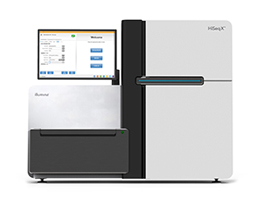
\includegraphics[width=.30\linewidth]{images/hiseq-x}};
                    \node (pro1) [process, below of=in1, yshift=-2.7cm] {Mapper};
                    \node (pro1_capt) [left of=pro1, xshift=-8.5cm] {BWA MEM 0.7.10};
                    \node (pro2) [process, below of=pro1] {Fix Mate Pairing};
                    \node (pro2_capt) [left of=pro2, xshift=-8.5cm] {Samtools 1.1 fixmates};
                    \node (pro3) [process, below of=pro2] {Sort};
                    \node (pro3_capt) [left of=pro3, xshift=-8.5cm] {Samtools 1.1 sort};
                    \node (pro4) [process, below of=pro3] {Mark Duplicates};
                    \node (pro4_capt) [left of=pro4, xshift=-8.5cm] {Picard 1.119 MarkDuplicates};
                    \node (pro4a) [process, below of=pro4] {Downsample};
                    \node (pro4a_capt) [left of=pro4a, xshift=-8.5cm] {Picard 1.119 DownsampleSam};
                    \node (pro5) [process, below of=pro4a] {Call};
                    \node (pro5_capt) [left of=pro5, xshift=-8.5cm] {Samtools 1.1 or GATK HC 1.1};
                    \node (pro6) [process, below of=pro5] {Normalise variants};
                    \node (pro6_capt) [left of=pro6, xshift=-8.5cm] {Bcftools 1.1 norm};
                    \node (dec1) [decision, below of=pro6, yshift=-1.5cm] {Evaluate};
                    \node (dec1_capt) [left of=dec1, xshift=-8.5cm] {Bcftools 1.1 stat};
                    \draw [arrow] (in1) -- (pro1);
                    \draw [arrow] (pro1) -- (pro2);
                    \draw [arrow] (pro2) -- (pro3);
                    \draw [arrow] (pro3) -- (pro4);
                    \draw [arrow] (pro4) -- (pro4a);
                    \draw [arrow] (pro4a) -- (pro5);
                    \draw [arrow] (pro5) -- (pro6);
                    \draw [arrow] (pro6) -- (dec1);
                \end{tikzpicture}
            \end{block}
            \begin{block}{What has changed?}
                \begin{itemize} \itemindent50pt
                    \item Error Profile (particularly context specific errors).
                    \item Quality Score Binning by default.
                    \item Read length increased to 150bp.
                    \item New Mappers available and required to take advantage of read length.
                \end{itemize}
            \end{block}
            \begin{block}{Method}
              In order to test the importance of the reference on our data we tested: 
                \begin{itemize} \itemindent80pt
                    \item 1000 Genomes Phase II reference - hs37d5
                    \item GRCh38 analysis reference without alts.
                \end{itemize}
              And the following callers:
                \begin{itemize} \itemindent80pt
                    \item Samtools and BCFtools 1.1
                    \item GATK Haplotype Caller 3.2
                \end{itemize}
              These were evaluated against:
                \begin{itemize} \itemindent80pt
                    \item NIST Genome in a Bottle 0.2 [1] (+ lifted over to GRCh38)
                \end{itemize}
                Additionally we downsampled the data using Picard 1.119 DownsampleSam from 30x to 5x in 2.5x intervals to explore the effects of various rates of coverage should the platform be opened to this in the future.
            \end{block}
            \begin{block}{Results}
            \begin{table}[h]
\begin{tabular}{|l|c|c|}
\hline
Sample  & Total SNPs Called & Hets \\ \cline{1-3} % & Hets from LCR & nRef Hom from LCR %
CHM1 & 2,897,438 & 294,267  \\ \cline{1-3} %& 15665 & 78062%
HAP1 & 2,943,962 & 324,009 \\ \cline{1-3} %& 16684 & 78080%
Mix & 4,060,909 & 2,598,304   \\ \cline{1-3} % & &%
\hline
\end{tabular}
\caption{Sites called for haploid samples across whole genome}
\label{table:1}
\end{table}

            \end{block}
            \vfill
          % ---------------------------------------------------------%
          % end the column

            \end{minipage}
        \end{beamercolorbox}
    \end{column}
        \begin{column}{.49\textwidth}
        \begin{beamercolorbox}[center,wd=\textwidth]{postercolumn}
            \begin{minipage}[T]{.95\textwidth}  % tweaks the width, makes a new \textwidth


            \begin{block}{Results (continued)}
            \begin{table}[h]
\begin{tabular}{|l|l|c|c|c|}
\hline
Ref & Pipeline & Called (TP) & In GIAB(FP) & Not Called (FN) \\ \cline{1-5}
38 & Replicate 1 Samtools 1.1 & 62919 & 2937 & 701 \\ \cline{1-5}
38 & Replicate 2 Samtools 1.1 & 62895 & 2890 & 725 \\ \cline{1-5}
38 & Replicate 1 GATK HC 3.2 & 62883 & 2911 & 737 \\ \cline{1-5}
38 & Replicate 2 GATK HC 3.2 & 62824 & 2768 & 796 \\ \cline{1-5}
38 & Illm Plat GATK HC 3.2 & 62878 & 2792 & 742 \\ \cline{1-5}
37 & Replicate 1 Samtools 1.1 & 63249 & 2721 & 703 \\ \cline{1-5}
37 & Replicate 2 Samtools 1.1 & 63224 & 2686 & 728 \\ \cline{1-5}
37 & Replicate 1 GATK HC 3.2 & 63211 & 2693 & 741 \\ \cline{1-5}
37 & Replicate 2 GATK HC 3.2 & 63153 & 2585 & 799 \\ \cline{1-5}
\hline
\end{tabular}
\caption{Call Rates for SNPs on NA12878 vs GIAB 0.2 in Highly Confident Areas of Genome on chr20}
\label{table:2}
\end{table}

            \begin{table}[h]
\begin{tabular}{|l|l|c|c|c|c|}
\hline
Ref & Set A & Set B & A Only & B Only & Intersect \\ \cline{1-6}
38 & Rep 1 Samtools & Rep 2 Samtools & 5316 & 4823 & 104884 \\ \cline{1-6}
38 & Rep 1 GATK & Rep 2 GATK & 6318 & 4942 & 101376 \\ \cline{1-6}
38 & Rep 1 GATK & Rep 1 Samtools&6880&9386&100814 \\ \cline{1-6}
38 & Rep 2 GATK & Rep 2 Samtools&6155&9544&100163 \\ \cline{1-6}
38 & Rep 2 GATK & Illumina Platinum&7175&8473&99143 \\ \cline{1-6}
\end{tabular}
\caption{Intersection of called sites on chr20}
\end{table}

                Perhaps surprisingly the difference between replicates appears to be as large as between callers.
                
                \begin{figure}
                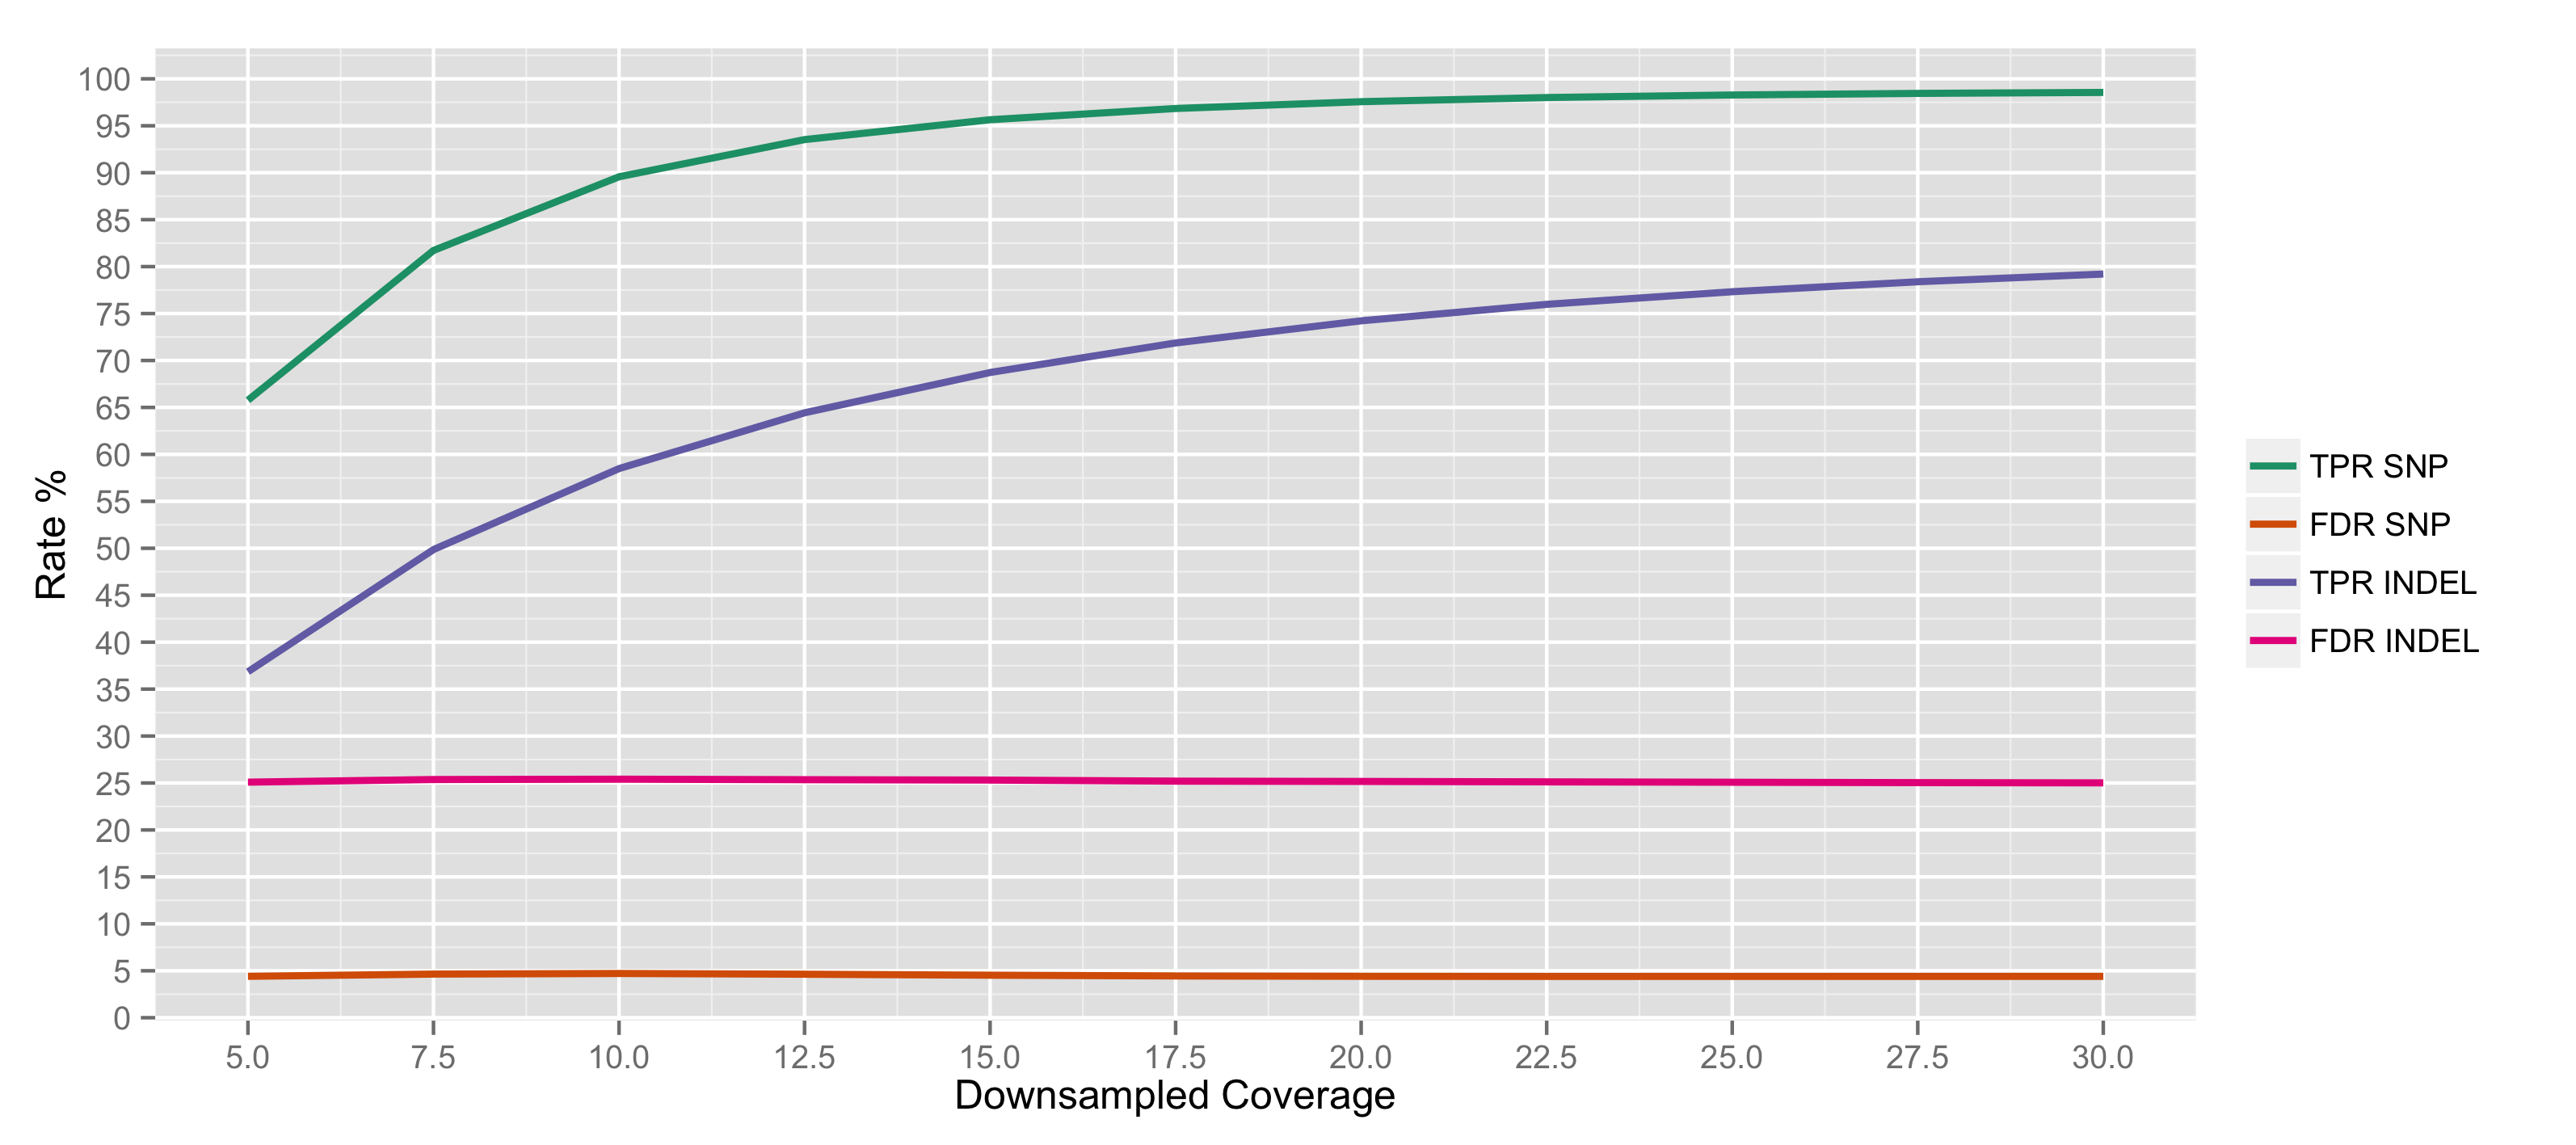
\includegraphics[width=0.95\textwidth]{images/downsampling_fig1}
                \caption{Rate of discovery of GIAB Genome Wide vs Downsampling Rate}
                \end{figure}

                The downsampling analysis showed that whilst the FDR seems to remain constant by coverage at approximately 4 and 25 percent for SNPs and INDELs respectively, the number of variants discovered at increased depth decreases at an exponential rate.  Whilst approximately 15x seems to be capture more than 96\% of SNPs with only a small improvement at higher depths of coverage it only captures 69\% of INDELs and additional depth can improve these slightly.

            \end{block}
            \begin{block}{Conclusions}
                The Illumina HiSeq X is a viable sequencing platform for our purposes and our proposed pipeline calls variants at an acceptable rate.  Our downsampling analysis suggests that for studies that are only interested in SNPs, the full coverage of a HiSeq X may be excessive but for discovering INDELs it is invaluable. Unfortunately the false discovery rate for INDELs remains high and suggests that our tools for these still need improvement in this respect. Since this work was started a new version of BWA has been proposed that supports mapping to alternate haplotypes, we plan to extend our analysis to incorporate an evaluation of the effects of mapping to these additional sequences.
            \end{block}
            \begin{block}{Acknowledgements}
                The Sanger's NPG and Sequencing R\&D Team for providing the data. Joshua Randall for help with Graphs and R. Thomas Keene for editorial guidance.
            \end{block}
            \begin{block}{References}
                [1] Zook, Justin M., Brad Chapman, Jason Wang, David Mittelman, Oliver Hofmann, Winston Hide, and Marc Salit. "Integrating Human Sequence Data Sets Provides a Resource of Benchmark Snp and Indel Genotype Calls." Nat Biotech 32, no. 3 (03//print 2014): 246-51.
            \end{block}
            \vfill

          % ---------------------------------------------------------%
          % end the column

            \end{minipage}
        \end{beamercolorbox}
    \end{column}
    \end{columns}

\end{frame}
\end{document}

